\documentclass[a4paper,11pt]{article}

\usepackage{amsmath}
\usepackage[pdftex]{graphicx}

\usepackage[english,greek]{babel}

\usepackage{lmodern}

\usepackage{listings}

\lstset{
  basicstyle=\ttfamily,
  columns=fullflexible,
  frame=single,
  breaklines=true
}

% Αφαίρεσε (Εισήγαγε) την παρακάτω γραμμή σε σχόλιο αν ο επεξεργαστής κειμένου (δεν) χρησιμοποιεί κωδικοποίηση Unicode για Ελληνικά
\usepackage[utf8x]{inputenc}

% Αφαίρεσε (Εισήγαγε) την παρακάτω γραμμή σε σχόλιο αν ο επεξεργαστής κειμένου (δεν) χρησιμοποιεί κωδικοποίηση iso-8859-7 για Ελληνικά
%\usepackage[iso-8859-7]{inputenc}

%Δημιουργία συντομεύσεων για αλλαγή γραφής σε Ελληνικά/Αγγλικά
\newcommand{\lt}{\latintext}
\newcommand{\gt}{\greektext}

\title{2η Υποχρεωτική Εργασία \\ Στο Μάθημα της Αριθμητικής Ανάλυσης: \\ Άσκηση 5}
\author{Ονοματεπώνυμο: Μπαρακλιλής Ιωάννης  \\  ΑΕΜ: 3685}
\date{4 Ιανουαρίου 2021}

\begin{document}

\maketitle
\section{Πολυωνυμική προσέγγιση}
Ζητείται να γίνει προσέγγιση του ημίτονου με πολυώνυμο χρησιμοποιώντας 10 τιμές του. Έχοντας αυτές τις τιμές δεδομένες, υπάρχει μοναδικό πολυώνυμο (το πολύ 9ου βαθμού) που επαληθεύει αυτά τα σημεία και μπορεί να βρεθεί με διάφορες μεθόδους. Επιλέγω να χρησιμοποιήσω την μέθοδο εύρεσης πολυώνυμου {\lt Newton}.

Για την επιλογή των 10 σημείων, επιλέγω 10 σημεία, με την ακρίβεια τιμής του ημίτονου στα 6 δεκαδικά ψηφία, ομοιόμορφα κατανεμημένα στο διάστημα $[-\pi, \pi]$ τα οποία είναι:
\begin{enumerate}
    \item {\lt $x = -\pi$} με {\lt $sin(x) = 0$}, δηλαδή το σημείο $(-\pi, 0)$
    \item {\lt $x = -\dfrac{7}{9}\pi$} με {\lt $sin(x) = -0.642788$}, δηλαδή το σημείο $(-\dfrac{7}{9}\pi, -0.642788)$
    \item {\lt $x = -\dfrac{5}{9}\pi$} με {\lt $sin(x) = -0.984808$}, δηλαδή το σημείο $(-\dfrac{5}{9}\pi, -0.984808)$
    \item {\lt $x = -\dfrac{\pi}{3}$} με {\lt $sin(x) = -\dfrac{\sqrt{3}}{2} \simeq -0.866025$}, δηλαδή το σημείο $(-\dfrac{\pi}{3}, -0.866025)$
    \item {\lt $x = -\dfrac{\pi}{9}$} με {\lt $sin(x) = -0.342020$}, δηλαδή το σημείο $(-\dfrac{\pi}{9}, -0.342020)$
    \item {\lt $x = \dfrac{\pi}{9}$} με {\lt $sin(x) = 0.342020$}, δηλαδή το σημείο $(\dfrac{\pi}{9}, 0.342020)$
    \item {\lt $x = \dfrac{\pi}{3}$} με {\lt $sin(x) = \dfrac{\sqrt{3}}{2} \simeq 0.866025$}, δηλαδή το σημείο $(\dfrac{\pi}{3}, 0.866025)$
    \item {\lt $x = \dfrac{5}{9}\pi$} με {\lt $sin(x) = 0.984808$}, δηλαδή το σημείο $(\dfrac{5}{9}\pi, 0.984808)$
    \item {\lt $x = \dfrac{7}{9}\pi$} με {\lt $sin(x) = 0.642788$}, δηλαδή το σημείο $(\dfrac{7}{9}\pi, 0.642788)$
    \item {\lt $x = \pi$} με {\lt $sin(x) = 0$}, δηλαδή το σημείο $(\pi, 0)$
\end{enumerate}

Το ζητούμενο υλοποιείται προγραμματιστικά στην γλώσσα {\lt python} (3.7) στο αρχείο με όνομα {\lt a\textunderscore polynomial\textunderscore approximation.py} το οποίο φαίνεται παρακάτω:
\lt
\lstinputlisting[language=Python]{a_polynomial_approximation.py}
\gt

\par
Στον παραπάνω κώδικα:\\
\par
Αρχικά, εισάγονται (γίνονται {\lt import}) τα {\lt sin, pi} απο την βιβλιοθήκη {\lt math} που θα χρειαστούν στην συνέχεια.\\

\par
Μετά, ορίζεται η συνάρτηση {\lt polynomial\textunderscore approximate} η οποία δέχεται ως όρισμα έναν δισδιάστο πίνακα όπου η κάθε γραμμή του αποτελεί ένα σημείο όπου στην πρώτη στήλη υπάρχει το {\lt $x$} και στην άλλη το {\lt $y$} και επιστρέφει έναν μονοδιάστατο πίνακα με τους συντελεστές του πολυωνύμου που περνάει από αυτά τα σημεία και το κάθε στοιχείο που περιέχει αποτελεί τον συντελεστή στην αντίστοιχή θέση (δηλαδή το πρώτο στοιχείο (θέση 0) του πίνακα αντιστοιχεί στην σταθερά, το δεύτερο (θέση 1) αντιστοιχεί στον συντελεστή του {\lt $x$}, το τρίτο (θέση 2), εφόσον το πολυώνυμο είναι δευτέρου βαθμού στον συντελεστή του {\lt $x^2$}, κ.ο.κ.).\\
Ανάλυση της λειτουργίας της:\\
Αρχικά, αντιγράφω τα {\lt $x, y$} των σημείων σε ξεχωριστούς (νέους) πίνακες {\lt x, y} αντίστοιχα.\\
Στην συνέχεια, ταξινομώ τους πίνακες {\lt x, y} ως ζεύγη (εφόσον είναι προϋπόθεση στην κατασκευή διαρεμένων διαφορών η ταξινόμηση των {\lt x}) με βάση το {\lt x} (ουσιαστικά ταξινομώ τα {\lt x} και τα {\lt y} αλλάζουν θέσεις σε αντιστοιχία με τα {\lt x}) χρησιμοποιώντας την συνάρτηση {\lt sort\textunderscore xy\textunderscore pairs} που ορίζεται πιο κάτω.\\
Μετά, υπολογίζω τον πίνακα διαιρεμένων διαφορών (που αποθηκεύεται στον πίνακα με όνομα {\lt temp\textunderscore dd}) υπολογίζοντας αρχικά τις διαιρεμένες διαφορές πρώτης τάξης (που εξαρτάται απο το {\lt y}) και μετά των επομένων τάξεων (που εξαρτώνται από τις προηγούμενης τάξης διαιρεμένες διάφορές) σύμφωνα με την θεωρία.\\
Στην συνέχεια, ορίζω τον πίνακα {\lt x\textunderscore coefficients} που θα αποθηκεύει τους συντελεστές του πολυωνύμου, και αρχικά έχει 0 σε κάθε θέση του εφόσον θα προστίθενται στην συνέχεια οι συντελεστές κάθε βήματος.\\
Επίσης ορίζω τον βοηθητικό πίνακα {\lt x\textunderscore minus\textunderscore xi\textunderscore coefficients} που αποθηκεύει τους συντελεστές του πολυωνύμου (η θέση του κάθε στοιχείου αντιστοιχεί στον συντελεστή της αντίστοιχης δύναμης του {\lt $x$}) που σχηματίζεται από το γινόμενο {\lt $\prod_{i=1}^{j}(x-x_{i-1})$} όπου {\lt $x_i$} είναι το {\lt $x$} του {\lt i}-ου σημείου και το {\lt j} είναι το βήμα του αλγορίθμου στο οποίο βρισκόμαστε (αρχικά (βήμα 0) ο πίνακας έχει τιμή 1 στο πρώτο στοιχείο και 0 στα υπόλοιπα του και στην συνέχεια τους συντελεστές του παραπάνω γινομένου). Για την υπολογισμό των περιεχομένων του (σε κάθε βήμα) αρκεί να θέσουμε ως νέα στοιχεία του τα μετατοπισμένα κατά μία θέση δεξιά στοιχεία του πίνακα του προηγουμένου βήματος (το πρώτο στοιχείο του νέου πίνακα θεωρούμε 0 και το τελευταίο του μετατοπισμένου πίνακα αγνοείται) και να αφαιρέσουμε τα στοιχεία της ίδιας θέσης πολλαπλασιασμένα κατά το {\lt $x_i$} ({\lt $i = $} βήμα - 1) (δηλαδή στο βήμα 0 έχουμε ότι ο πίνακας έχει τιμή 1 στο πρώτο στοιχείο και 0 στα υπόλοιπα, στο βήμα 1 θα έχει {\lt $-x_0$} στο πρώτο στοιχείο, 1 στο δεύτερο και 0 στα υπόλοιπα, στο βήμα 2 θα έχει {\lt $(-x_0)\cdot (-x_1)$} στο πρώτο στοιχείο, {\lt $-x_0 - (x_1)$} στο δεύτερο, 1 στο τρίτο και 0 στα υπόλοιπα,  κ.ο.κ. για τα υπόλοιπα βήματα). Αυτό εξηγείται ως εξής: αρχικά έχουμε 1 στο πρώτο στοιχείο και 0 στα υπόλοιπα δηλαδή το πολυώνυμο 1, την συνέχεια αν πολλαπλασιάσουμε το προηγούμενο με {\lt $(x - x_0)$} τότε έχουμε το πολυώνυμο {\lt $1\cdot (x-x_0) = -x_0 + x$} δηλαδή το πολυώνυμο με συντελεστές τα {\lt $-x_0$} και 1, στην συνέχεια αν πολλαπλασιάσουμε το προηγούμενο με {\lt $(x - x_1)$} έχουμε το πολυώνυμο {\lt $(x - x_0)\cdot (x - x_1) = x^2 + x\cdot (-x_1) + (-x_0)\cdot x + (-x_0)\cdot (-x_1) = (-x_0)\cdot (-x_1) + (-x_1 -x_0)x + x^2 $} δηλαδή το πολυώνυμο με συντελεστές τα {\lt $(-x_0)\cdot (-x_1)$}, {\lt $-x_0 - (x_1)$} και 1, κ.ο.κ. για τα επόμενα βήματα. Επομένως, βλέπουμε ότι μπορεί με αυτόν τον τρόπο να υπολογιστούν οι συντελεστές του γινομένου αυτού.\\
Ακολούθως, αρχίζει ένας βρόχος στον οποίο: Αρχικά, ορίζεται ο πίνακας {\lt x\textunderscore minus\textunderscore xi\textunderscore coefficients\textunderscore new} που έχει αρχικά σε κάθε θέση 0 και την συνέχεια υπολογίζονται σύμφωνα με την παραπάνω διαδικασία και αποθηκεύονται σε αυτόν οι συντελεστές του πολυωνύμου του γινομένου {\lt $\prod_{i=1}^{j}(x-x_{i-1})$} του επομένου βήματος. Τέλος, προστίθεται στον πίνακα {\lt x\textunderscore coefficients} ο πίνακας {\lt x\textunderscore minus\textunderscore xi\textunderscore coefficients\textunderscore new} πολλαπλασιασμένος με την πρώτη διαιρεμένη διαφορά της τάξης ίδιας με του βήματος.\\
Σύμφωνα με τα παραπάνω, μπορεί κάποιος να διαπιστώσει ότι αφού τερματίσει ο βρόχος στον πίνακα {\lt x\textunderscore coefficients} θα βρίσκονται οι συντελεστές του πολυωνύμου που διέρχεται από τα σημεία που δίνονται ως όρισμα.
Τέλος, επιστρέφεται ο πίνακας {\lt x\textunderscore coefficients}.\\

\par
Στην συνέχεια, ορίζεται η συνάρτηση {\lt sort\textunderscore xy\textunderscore pairs} η οποία δέχεται δύο πίνακες και ταξινομεί επί τόπου ({\lt in place}) τα στοιχεία τους ως ζεύγη βάσει των στοιχείων του πρώτου πίνακα με την μέθοδο της ταξινόμησης με επιλογή. Δηλαδή, ταξινομεί τον πρώτο πίνακα και κάθε ανταλλαγή στοιχείων που γίνεται στον πρώτο γίνεται η αντίστοιχη και στον δεύτερο.\\

\par
Ακολούθως, ορίζεται η συνάρτηση {\lt calculate\textunderscore polynomial} η οποία δέχεται έναν πίνακα συντελεστών πολυωνύμου (όπου η θέση κάθε στοιχείου αντιστοιχεί στην δύναμη του αγνώστου) και έναν (πραγματικό) αριθμό {\lt x} και υπολογίζει και επιστρέφει την τιμή του πολυωνύμου για το δοθέν σημείο.\\

\par
Μετά, ορίζεται η συνάρτηση {\lt sin\textunderscore approximation} η οποία δέχεται έναν (πραγματικό) αριθμό {\lt x} και υπολογίζει και επιστρέφει το ημίτονο της δοθείσας γωνίας {\lt x} χρησιμοποιώντας πολυωνυμική προσέγγιση με βάση τα παραπάνω σημεία. Αυτή η συνάρτηση για τον υπολογισμό της προσέγγισης του ημίτονου χρησιμοποιεί τις παραπάνω συναρτήσεις. Για τον υπολογισμό του ημίτονου αρκεί κάποιος να εκτελέσει αυτή την συνάρτηση για κάποια γωνία.\\

\par
Τέλος, ορίζεται η συνάρτηση {\lt main}, η οποία δεν δέχεται ορίσματα, η οποία θα εκτελεστεί όταν εκτελεστεί το αρχείο στο οποίο αναφερόμαστε και για τα σημεία που επέλεξα παραπάνω υπολογίζει μέσω την πολυωνυμικής προσέγγισης και εμφανίζει  (εμφάνιση με ακρίβεια 6 δεκαδικών ψηφίων) το ημίτονο στα παραπάνω σημεία και εμφανίζει το απόλυτο σφάλμα από το πραγματικό ημίτονο, χρησιμοποιώντας την συνάρτηση {\lt sin} από την βιβλιοθήκη {\lt math}.\\

\par
Αν εκτελέσουμε το αρχείο θα τυπωθεί στην οθόνη το ακόλουθο:\\
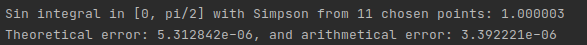
\includegraphics[width=\linewidth]{Exercise5/run_a.png}\\

Παραπάνω, βλέπουμε ότι για:
\begin{itemize}
    \item {\lt $x = -\pi$} έχω προσέγγιση έχω προσέγγιση 0.000000 και απόλυτο σφάλμα $1.454732 \cdot 10^{-15}$
    \item {\lt $x = -\dfrac{7}{9}\pi$} έχω προσέγγιση -0.642788 και απόλυτο σφάλμα $3.903135\cdot 10^{-7}$
    \item {\lt $x = -\dfrac{5}{9}\pi$} έχω προσέγγιση -0.984808 και απόλυτο σφάλμα $2.469878\cdot 10^{-7}$
    \item {\lt $x = -\dfrac{\pi}{3}$} έχω προσέγγιση -0.866025 και απόλυτο σφάλμα $4.037844\cdot 10^{-7}$
    \item {\lt $x = -\dfrac{\pi}{9}$} έχω προσέγγιση -0.342020 και απόλυτο σφάλμα $1.433257\cdot 10^{-7}$
    \item {\lt $x = \dfrac{\pi}{9}$} έχω προσέγγιση 0.342020 και απόλυτο σφάλμα $1.433257\cdot 10^{-7}$
    \item {\lt $x = \dfrac{\pi}{3}$} έχω προσέγγιση 0.866025 και απόλυτο σφάλμα $4.037844\cdot 10^{-7}$
    \item {\lt $x = \dfrac{5}{9}\pi$} έχω προσέγγιση 0.984808 και απόλυτο σφάλμα $2.469878\cdot 10^{-7}$
    \item {\lt $x = \dfrac{7}{9}\pi$} έχω προσέγγιση 0.642788 και απόλυτο σφάλμα $3.903135\cdot 10^{-7}$
    \item {\lt $x = \pi$} έχω προσέγγιση 0.000000 και απόλυτο σφάλμα $2.958404\cdot 10^{-15}$
\end{itemize}

Επομένως, στα <<γνωστά>> σημεία, έχουμε μεγαλύτερο απόλυτο σφάλμα για {\lt $x = -\dfrac{\pi}{3}, x = \dfrac{\pi}{3}$}  με σφάλμα $4.037844\cdot 10^{-7} = 0.4037844\cdot 10^{-8}  < \dfrac{1}{2}10^{-8}$, επομένως στα <<γνωστά>> σημεία έχουμε ακρίβεια τουλάχιστον 8 δεκαδικών ψηφίων.

\par
Αν στην συνέχεια πάρουμε 200 σημεία ομοιόμορφα κατανεμημένα στο $[-\pi, \pi]$, υπολογίσουμε το απόλυτο σφάλμα, και εμφανίσουμε το σφάλμα αυτό κάθε σημείου σε διάγραμμα, έχουμε το παρακάτω (υπολογίστηκε χρησιμοποιώντας την συνάρτηση {\lt scatter} του {\lt pyplot} της βιβλιοθήκης {\lt matplotlib} στο αρχείο {\lt a\textunderscore polynomial\textunderscore approximation\textunderscore errors\textunderscore graph.py} που περιλαμβάνει τον ίδιο κώδικα με το αρχείο που περιγράφεται παραπάνω με διαφορετική όμως {\lt main} που αντί να χρησιμοποιεί τα δεδομένα σημεία, <<επιλέγει>> ομοιόμορφα κατανεμημένα 200 σημεία στο $[-\pi, \pi]$, υπολογίζει τις προσεγγίσεις κάθε ενός από τα αυτά και κατασκευάζει το διάγραμμα):\\

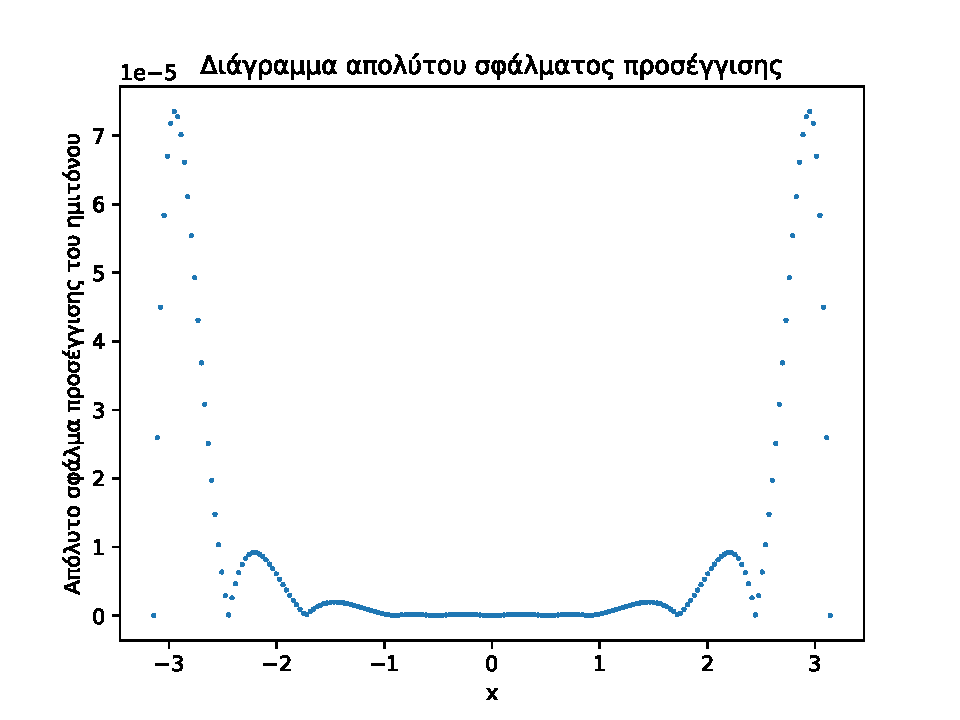
\includegraphics[width=\linewidth]{Exercise5/Figure_a.pdf}\\
Από το παραπάνω διάγραμμα μπορούμε να δούμε ότι στα 200 σημεία το απόλυτο σφάλμα δεν ξεπερνάει το $8\cdot 10^{-5} = 0.8\cdot 10^{-6} < \dfrac{1}{2}10^{-5}$. Επομένως, σε αυτά τα 200 σημεία έχουμε τουλάχιστον 5 δεκαδικά ψηφία ακρίβειας.

\section{Προσέγγιση με {\lt Splines}}
Ζητείται να γίνει προσέγγιση του ημίτονου με {\lt splines} χρησιμοποιώντας 10 τιμές του. Όπως και στην περίπτωση της πολυωνυμικής προσέγγισης για την επιλογή των 10 σημείων, επιλέγω 10 σημεία, με την ακρίβεια τιμής του ημίτονου στα 6 δεκαδικά ψηφία, ομοιόμορφα κατανεμημένα στο διάστημα $[-\pi, \pi]$ τα οποία είναι:
\begin{enumerate}
    \item {\lt $x = -\pi$} με {\lt $sin(x) = 0$}, δηλαδή το σημείο $(-\pi, 0)$
    \item {\lt $x = -\dfrac{7}{9}\pi$} με {\lt $sin(x) = -0.642788$}, δηλαδή το σημείο $(-\dfrac{7}{9}\pi, -0.642788)$
    \item {\lt $x = -\dfrac{5}{9}\pi$} με {\lt $sin(x) = -0.984808$}, δηλαδή το σημείο $(-\dfrac{5}{9}\pi, -0.984808)$
    \item {\lt $x = -\dfrac{\pi}{3}$} με {\lt $sin(x) = -\dfrac{\sqrt{3}}{2} \simeq -0.866025$}, δηλαδή το σημείο $(-\dfrac{\pi}{3}, -0.866025)$
    \item {\lt $x = -\dfrac{\pi}{9}$} με {\lt $sin(x) = -0.342020$}, δηλαδή το σημείο $(-\dfrac{\pi}{9}, -0.342020)$
    \item {\lt $x = \dfrac{\pi}{9}$} με {\lt $sin(x) = 0.342020$}, δηλαδή το σημείο $(\dfrac{\pi}{9}, 0.342020)$
    \item {\lt $x = \dfrac{\pi}{3}$} με {\lt $sin(x) = \dfrac{\sqrt{3}}{2} \simeq 0.866025$}, δηλαδή το σημείο $(\dfrac{\pi}{3}, 0.866025)$
    \item {\lt $x = \dfrac{5}{9}\pi$} με {\lt $sin(x) = 0.984808$}, δηλαδή το σημείο $(\dfrac{5}{9}\pi, 0.984808)$
    \item {\lt $x = \dfrac{7}{9}\pi$} με {\lt $sin(x) = 0.642788$}, δηλαδή το σημείο $(\dfrac{7}{9}\pi, 0.642788)$
    \item {\lt $x = \pi$} με {\lt $sin(x) = 0$}, δηλαδή το σημείο $(\pi, 0)$
\end{enumerate}
Επίσης, επιλέγω να υπολογιστεί ως {\lt spline} η φυσική κυβική {\lt spline}

Το ζητούμενο υλοποιείται προγραμματιστικά στην γλώσσα {\lt python} (3.7) στο αρχείο με όνομα {\lt b\textunderscore splines\textunderscore approximation.py} το οποίο φαίνεται παρακάτω:
\lt
\lstinputlisting[language=Python]{b_splines_approximation.py}
\gt

\par
Στον παραπάνω κώδικα:\\
\par
Αρχικά, εισάγονται (γίνονται {\lt import}) τα {\lt sin, pi} απο την βιβλιοθήκη {\lt math} που θα χρειαστούν στην συνέχεια.\\

\par
Μετά, ορίζεται η συνάρτηση {\lt splines\textunderscore approximate} που δέχεται ως όρισμα έναν δισδιάστο πίνακα όπου η κάθε γραμμή του αποτελεί ένα σημείο όπου στην πρώτη στήλη υπάρχει το {\lt $x$} και στην άλλη το {\lt $y$} και επιστρέφει
έναν δισδιάστατο πίνακα όπου η κάθε γραμμή του αντιστοιχεί σε φυσική κυβική {\lt spline} ενός διαστήματος. Σε αυτόν τον πίνακα που επιστρέφει, στο πρώτο στοιχείο της κάθε γραμμής υπάρχει ένας πίνακας δύο στοιχείων που θέτουν της αρχή και το τέλος του διαστήματος αντίστοιχα στο οποίο ορίζεται η {\lt spline} και στο δεύτερο στοιχείο κάθε γραμμής υπάρχει ένας πίνακας 4 θέσεων όπου τα στοιχεία του είναι οι συντελεστές του πολυωνύμου τρίτης τάξης της {\lt spline} στο αντίστοιχο διάστημα.\\
Αναλυτικά:\\
Αρχικά, ταξινομώ τα σημεία που δίνονται (απαιτείται για τον υπολογισμό της {\lt spline}) από το όρισμα με βάση το {\lt x} (ουσιαστικά ταξινομώ τα {\lt x} και τα {\lt y} αλλάζουν θέσεις σε αντιστοιχία με τα {\lt x}) χρησιμοποιώντας την συνάρτηση {\lt sort\textunderscore xy\textunderscore pairs} που ορίζεται πιο κάτω και αποθηκεύω τα ταξινομημένα σημεία στον πίνακα {\lt x\textunderscore y}.\\
Στην συνέχεια ορίζω ένα σύστημα {\lt 4n $\times$ 4n} όπου {\lt n} είναι ο αριθμός σημείων - 1 αρχικοποιώντας του πίνακες  
{\lt coefficients\textunderscore matrix} που αποθηκεύει τους συντελεστές των αγνώστων του συστήματος και {\lt constants\textunderscore matrix} που αποθηκεύει τις σταθερές του συστήματος, όπου οι δύο πίνακες αρχικά έχουν 0 σε κάθε τους θέση.\\
Το σύστημα αυτό έχει ως αγνώστους τους συντελεστές του πολυωνύμου τρίτης τάξης κάθε κλάδου της {\lt spline}. Έχουμε ότι για κάθε διάστημα {\lt $[x_i, x_{i+1}]$, $i = 1, ..., n$} (με {\lt n}+1 αριθμό σημείων ορίσματος όπου {\lt $n$} ο αριθμός των σημείων) έχουμε την φυσική κυβική {\lt spline} {\lt $s^{(i)}(x) = a^{(i)}x^3 + b^{(i)}x^2 + c^{(i)}x + d^{(i)}$}. Επομένως, εφόσον είναι δύο φορές παραγωγίσιμη, έχουμε {\lt $(s^{(i)})^{'}(x) = 3a^{(i)}x^2 + 2b^{(i)}x + c^{(i)}$} και {\lt $(s^{(i)})^{''}(x) = 6a^{(i)}x + 2b^{(i)} $}.
Κατασκευάζω αυτό το σύστημα ώστε να ισχύουν οι ακόλουθες συνθήκες της φυσικής κυβικής {\lt spline}:\\
\begin{itemize}    
    \item {\lt $s^{(i)}(x_{i}) = y_{i} \Longrightarrow a^{(i)}\cdot x_{i}^3 + b^{(i)}\cdot x_{i}^2 + c^{(i)}\cdot x_{i} + d^{(i)} = y_i$}, {\lt $\forall i = 0, ..., n$} με {\lt n}+1 αριθμό σημείων ορίσματος,
    \item {\lt $s^{(i-1)}(x_{i}) = s^{(i)}(x_i) =  y_{i} \Longrightarrow a^{(i-1)}\cdot x_{i}^3 + b^{(i-1)}\cdot x_{i}^2 + c^{(i-1)}\cdot x_{i} + d^{(i-1)} = y_i$},  {\lt $\forall i = 1, ..., n$} όπου {\lt n}+1 αριθμός σημείων ορίσματος,
    \item {\lt $(s^{(i-1)})^{'}(x_{i}) = (s^{(i)})^{'}(x_i) \Longrightarrow 3a^{(i-1)}x_{i}^2 + 2b^{(i-1)}x_{i} + c^{(i-1)} - 3a^{(i)}x_i^2 - 2b^{(i)}x_i - c^{(i)} = 0$}, {\lt $\forall i = 1, ..., n$} όπου {\lt n}+1 αριθμός σημείων ορίσματος,
    \item {\lt $(s^{(i-1)})^{''}(x_{i}) = (s^{(i)})^{''}(x_i) \Longrightarrow 6a^{(i-1)}x_{i} + 2b^{(i-1)} - 6a^{(i)}x_i - 2b^{(i)} = 0$}, {\lt $\forall i = 1, ..., n$} όπου {\lt n}+1 αριθμός σημείων ορίσματος,
    \item {\lt $(s^{(0)})^{''}(x_0) = 0 \Longrightarrow  6a^{(i)}x_0 + 2b^{(i)} = 0$} και 
    \item {\lt $(s^{(0)})^{''}(x_n) = 0 \Longrightarrow  6a^{(i)}x_n + 2b^{(i)} = 0$}.
\end{itemize}
Ακολούθως, λύνω το παραπάνω σύστημα με την συνάρτηση {\lt solve\textunderscore system} και χωρίζω το αποτέλεσμα σε πίνακες τεσσάρων στοιχείων (εφόσον έχω κυβική {\lt spline} κάθε τμήμα της είναι πολυώνυμο τρίτου βαθμού επομένως έχει τέσσερις συντελεστές), εισάγω αυτούς του πίνακες σε νέο δισδιάστατο πίνακα πίνακα που έχει αριθμό γραμμών ίσο με τον αριθμό των δοθέντων σημείων - 1 και στην πρώτη στήλη της κάθε γραμμής έχει έναν πίνακα δύο στοιχείων που περιέχει την αρχή και το τέλος του διαστήματος αντίστοιχα στο οποίο ορίζεται η {\lt spline} και στο δεύτερο στοιχείο κάθε γραμμής υπάρχει ένας ο πίνακας 4 θέσεων όπου τα στοιχεία του είναι οι συντελεστές του πολυωνύμου τρίτης τάξης της {\lt spline} στο αντίστοιχο διάστημα.\\

\par
Στην συνέχεια, ορίζω την συνάρτηση {\lt calculate\textunderscore spline} η οποία δέχεται έναν διασδιάστατο πίνακα με ίδια μορφή με αυτή του πίνακα που επιστρέφει η {\lt splines\textunderscore approximate} και έναν (πραγματικό) αριθμό {\lt x} και υπολογίζει και επιστρέφει την τιμή της {\lt spline} (του αντίστοιχου διαστήματος) για το δοθέν σημείο (αν δεν υπάρχει διάστημα το οποίο να περιέχει το δοθέν σημείο και να έχει υπολογιστεί {\lt Spline} σε αυτό, η συνάρτηση επιστέφει {\lt None}).\\

\par
Μετά, ορίζονται οι συναρτήσεις {\lt swap\textunderscore rows, pivot\textunderscore matrix, matrix\textunderscore vector\textunderscore multiplication, PLU, solve\textunderscore system} οι οποίες συνολικά έχουν την λειτουργία του να λύνουν ένα γραμμικό σύστημα με την μέθοδο {\lt PA = LU} χρησιμοποιώντας την συνάρτηση {\lt solve\textunderscore system} που δέχεται έναν πίνακα συντελεστών και ένα διάνυσμα (πίνακα στήλη) του συστήματος και επιστρέφει την λύση του συστήματος. Η υλοποίηση τους δεν ζητείται από την εκφώνηση και είναι (εκτός κάποιας διόρθωσης) πανομοιότυπες με εκείνες που ζητήθηκαν στο πρώτο υποερώτημα της τρίτης άσκησης της πρώτης υποχρεωτικής εργασίας, συνεπώς η ανάλυση τους παραλείπεται.\\

\par
Κατόπιν, ορίζεται η συνάρτηση {\lt sort\textunderscore xy\textunderscore pairs} η οποία δέχεται δύο πίνακες και ταξινομεί επί τόπου ({\lt in place}) τα στοιχεία τους ως ζεύγη βάσει των στοιχείων του πρώτου πίνακα με την μέθοδο της ταξινόμησης με επιλογή. Δηλαδή, ταξινομεί τον πρώτο πίνακα και κάθε ανταλλαγή στοιχείων που γίνεται στον πρώτο γίνεται η αντίστοιχη και στον δεύτερο. Είναι πανομοιότυπη με εκείνη του πρώτου ζητουμένου.\\

\par
Μετά, ορίζεται η συνάρτηση {\lt sin\textunderscore approximation} η οποία δέχεται έναν (πραγματικό) αριθμό {\lt x} και υπολογίζει και επιστρέφει το ημίτονο της δοθείσας γωνίας {\lt x} χρησιμοποιώντας προσέγγιση με {\lt splines} με βάση τα παραπάνω σημεία. Αυτή η συνάρτηση για τον υπολογισμό της προσέγγισης του ημίτονου χρησιμοποιεί τις παραπάνω συναρτήσεις (αν δεν υπάρχει διάστημα το οποίο να περιέχει το δοθέν σημείο και να έχει υπολογιστεί {\lt Spline} σε αυτό, η συνάρτηση επιστέφει {\lt None}). Για τον υπολογισμό του ημίτονου αρκεί κάποιος να εκτελέσει αυτή την συνάρτηση για κάποια γωνία.\\

\par
Τέλος, ορίζεται η συνάρτηση {\lt main}, η οποία δεν δέχεται ορίσματα, η οποία θα εκτελεστεί όταν εκτελεστεί το αρχείο στο οποίο αναφερόμαστε και για τα σημεία που επέλεξα παραπάνω υπολογίζει μέσω την προσέγγισης των (φυσικών κυβικών) {\lt splines} και εμφανίζει  (εμφάνιση με ακρίβεια 6 δεκαδικών ψηφίων) το ημίτονο στα παραπάνω σημεία και εμφανίζει το απόλυτο σφάλμα από το πραγματικό ημίτονο, χρησιμοποιώντας την συνάρτηση {\lt sin} από την βιβλιοθήκη {\lt math}.\\

\par
Αν εκτελέσουμε το αρχείο θα τυπωθεί στην οθόνη το ακόλουθο:\\
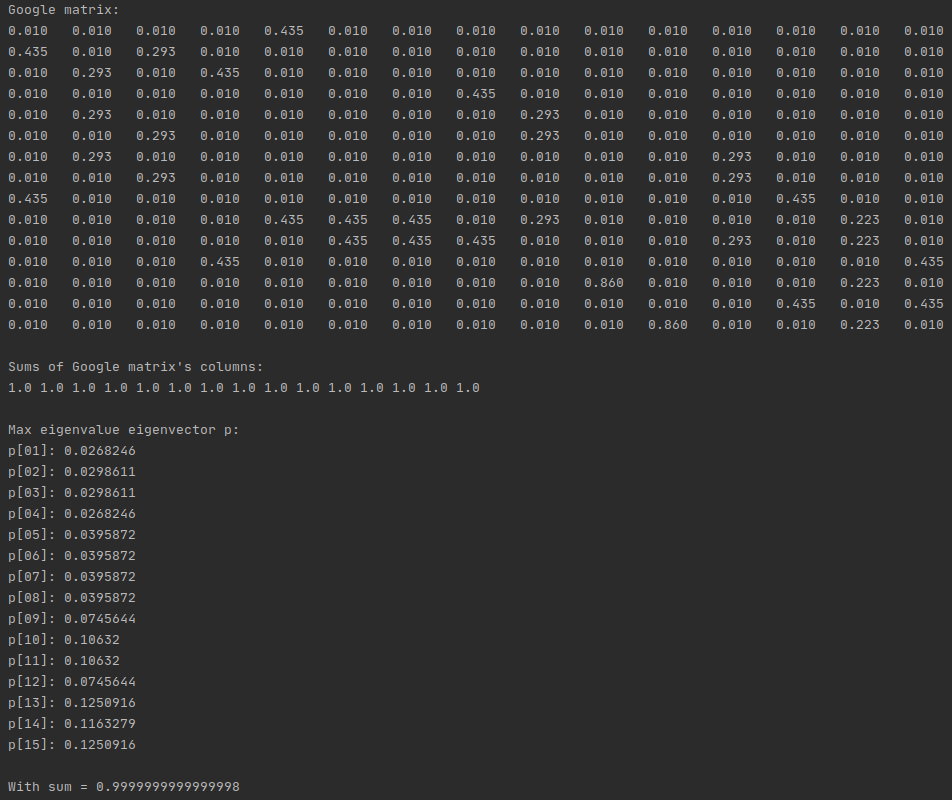
\includegraphics[width=\linewidth]{Exercise5/run_b.png}\\

Παραπάνω βλέπουμε ότι για:\\
\begin{itemize}
    \item {\lt $x = -\pi$} έχω προσέγγιση 0.000000 και απόλυτο σφάλμα $3.445093 \cdot 10^{-16}$
    \item {\lt $x = -\dfrac{7}{9}\pi$} έχω προσέγγιση -0.642788 και απόλυτο σφάλμα $3.903135 \cdot 10^{-7}$
    \item {\lt $x = -\dfrac{5}{9}\pi$} έχω προσέγγιση -0.984808 και απόλυτο σφάλμα $2.469878 \cdot 10^{-7}$
    \item {\lt $x = -\dfrac{\pi}{3}$} έχω προσέγγιση -0.866025 και απόλυτο σφάλμα $4.037844 \cdot 10^{-7}$
    \item {\lt $x = -\dfrac{\pi}{9}$} έχω προσέγγιση -0.342020 και απόλυτο σφάλμα $1.433257 \cdot 10^{-7}$
    \item {\lt $x = \dfrac{\pi}{9}$} έχω προσέγγιση 0.342020 και απόλυτο σφάλμα $1.433257 \cdot 10^{-7}$
    \item {\lt $x = \dfrac{\pi}{3}$} έχω προσέγγιση 0.866025 και απόλυτο σφάλμα $4.037844 \cdot 10^{-7}$
    \item {\lt $x = \dfrac{5}{9}\pi$} έχω προσέγγιση 0.984808 και απόλυτο σφάλμα $2.469878 \cdot 10^{-7}$
    \item {\lt $x = \dfrac{7}{9}\pi$} έχω προσέγγιση 0.642788 και απόλυτο σφάλμα $3.903135 \cdot 10^{-7}$
    \item {\lt $x = \pi$} έχω προσέγγιση 0.000000 και απόλυτο σφάλμα $5.665539 \cdot 10^{-16}$
\end{itemize}

Επομένως, στα <<γνωστά>> σημεία, έχουμε μεγαλύτερο απόλυτο σφάλμα για {\lt $x = -\dfrac{\pi}{3}, x = \dfrac{\pi}{3}$} με (απόλυτο) σφάλμα $4.037844 \cdot 10^{-7} = 0.4037844 \cdot 10^{-8} < \dfrac{1}{2}10^-8$, επομένως στα <<γνωστά>> σημεία έχουμε ακρίβεια τουλάχιστον 8 δεκαδικών ψηφίων.

\par
Αν στην συνέχεια πάρουμε 200 σημεία ομοιόμορφα κατανεμημένα στο $[-\pi, \pi]$, υπολογίσουμε το απόλυτο σφάλμα, και εμφανίσουμε το σφάλμα αυτό κάθε σημείου σε διάγραμμα έχουμε το παρακάτω (υπολογίστηκε χρησιμοποιώντας την συνάρτηση {\lt scatter} του {\lt pyplot} της βιβλιοθήκης {\lt matplotlib} στο αρχείο {\lt b\textunderscore splines\textunderscore approximation\textunderscore errors\textunderscore graph.py} που περιλαμβάνει τον ίδιο κώδικα με το αρχείο που περιγράφεται παραπάνω με διαφορετική όμως {\lt main} που αντί να χρησιμοποιεί τα δεδομένα σημεία, <<επιλέγει>> ομοιόμορφα κατανεμημένα 200 σημεία στο $[-\pi, \pi]$, υπολογίζει τις προσεγγίσεις κάθε ενός από τα αυτά και κατασκευάζει το διάγραμμα):\\

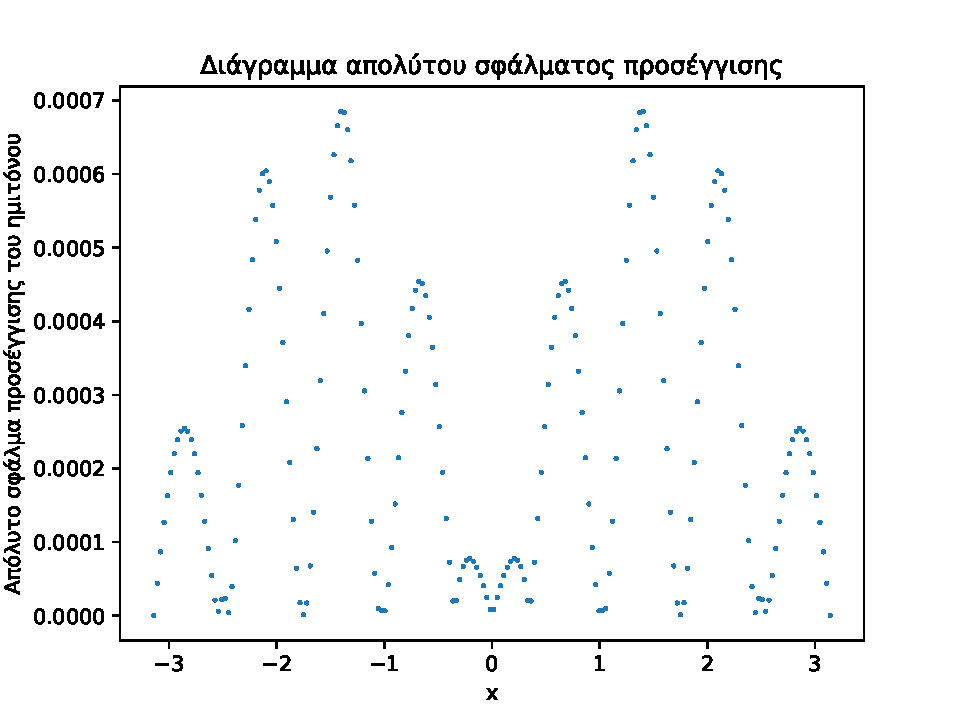
\includegraphics[width=\linewidth]{Exercise5/Figure_b.pdf}\\
Από το παραπάνω διάγραμμα μπορούμε να δούμε ότι στα 200 σημεία το απόλυτο σφάλμα δεν ξεπερνάει το $0.00008 < \dfrac{1}{2}10^{-3}$. Επομένως, σε αυτά τα 200 σημεία έχουμε τουλάχιστον 3 δεκαδικά ψηφία ακρίβειας.


\section{Προσέγγιση με ελάχιστα τετράγωνα}
Ζητείται να γίνει προσέγγιση του ημίτονου με ελάχιστα τετράγωνα χρησιμοποιώντας 10 τιμές του. Όπως και στην περίπτωση της πολυωνυμικής προσέγγισης για την επιλογή των 10 σημείων, επιλέγω 10 σημεία, με την ακρίβεια τιμής του ημίτονου στα 6 δεκαδικά ψηφία, ομοιόμορφα κατανεμημένα στο διάστημα $[-\pi, \pi]$ τα οποία είναι:
\begin{enumerate}
    \item {\lt $x = -\pi$} με {\lt $sin(x) = 0$}, δηλαδή το σημείο $(-\pi, 0)$
    \item {\lt $x = -\dfrac{7}{9}\pi$} με {\lt $sin(x) = -0.642788$}, δηλαδή το σημείο $(-\dfrac{7}{9}\pi, -0.642788)$
    \item {\lt $x = -\dfrac{5}{9}\pi$} με {\lt $sin(x) = -0.984808$}, δηλαδή το σημείο $(-\dfrac{5}{9}\pi, -0.984808)$
    \item {\lt $x = -\dfrac{\pi}{3}$} με {\lt $sin(x) = -\dfrac{\sqrt{3}}{2} \simeq -0.866025$}, δηλαδή το σημείο $(-\dfrac{\pi}{3}, -0.866025)$
    \item {\lt $x = -\dfrac{\pi}{9}$} με {\lt $sin(x) = -0.342020$}, δηλαδή το σημείο $(-\dfrac{\pi}{9}, -0.342020)$
    \item {\lt $x = \dfrac{\pi}{9}$} με {\lt $sin(x) = 0.342020$}, δηλαδή το σημείο $(\dfrac{\pi}{9}, 0.342020)$
    \item {\lt $x = \dfrac{\pi}{3}$} με {\lt $sin(x) = \dfrac{\sqrt{3}}{2} \simeq 0.866025$}, δηλαδή το σημείο $(\dfrac{\pi}{3}, 0.866025)$
    \item {\lt $x = \dfrac{5}{9}\pi$} με {\lt $sin(x) = 0.984808$}, δηλαδή το σημείο $(\dfrac{5}{9}\pi, 0.984808)$
    \item {\lt $x = \dfrac{7}{9}\pi$} με {\lt $sin(x) = 0.642788$}, δηλαδή το σημείο $(\dfrac{7}{9}\pi, 0.642788)$
    \item {\lt $x = \pi$} με {\lt $sin(x) = 0$}, δηλαδή το σημείο $(\pi, 0)$
\end{enumerate}
Επίσης, επιλέγω η προσέγγιση αυτή να γίνει με πολυώνυμο δευτέρου βαθμού.

Το ζητούμενο υλοποιείται προγραμματιστικά στην γλώσσα {\lt python} (3.7) στο αρχείο με όνομα {\lt c\textunderscore least\textunderscore squares\textunderscore approximation.py} το οποίο φαίνεται παρακάτω:
\lt
\lstinputlisting[language=Python]{c_least_squares_approximation.py}
\gt

\par
Στον παραπάνω κώδικα:\\
\par
Αρχικά, εισάγονται (γίνονται {\lt import}) τα {\lt sin, pi} απο την βιβλιοθήκη {\lt math} που θα χρειαστούν στην συνέχεια.\\

\par
Στην συνέχεια, ορίζω την συνάρτηση {\lt least\textunderscore squares} η οποία δέχεται έναν πίνακα συντελεστών {\lt A} και ένα διάνυσμα (πίνακα στήλη) σταθερών {\lt b} και επιστρέφει την λύση του συστήματος με ελάχιστα τετράγωνα.\\
Αναλυτικά:\\
Αρχικά, αναστρέφεται ο πίνακας Α (με την συνάρτηση {\lt matrix\textunderscore transposition} που ορίζεται αργότερα) και ο ανάστροφος αυτός πολλαπλασιάζει απο τα αριστερά τον πίνακα {\lt A} και το διάνυσμα {\lt b} του ορίσματος (με τις συναρτήσεις {\lt matrix\textunderscore multiplication} {\lt matrix\textunderscore vector\textunderscore multiplication} που εκτελούν πολλαπλασιασμό πινάκων και πολλαπλασιασμό πίνακα με διάνυσμα (πίνακα στήλη) αντίστοιχα και επιστρέφουν το αποτέλεσμα και οι οποίες ορίζονται παρακάτω) και χρησιμοποιώ τα αποτελέσματα των γινομένων ως πίνακα συντελεστών και διάνυσμα σταθερών ενός συστήματος το οποίο λύνω (με την συνάρτηση {\lt solve\textunderscore system} που ορίζεται παρακάτω) και επιστρέφω το αποτέλεσμα το οποίο είναι η λύση ελαχίστων τετραγώνων του συστήματος.\\

\par
Ακολούθως, ορίζω την συνάρτηση {\lt approximate\textunderscore function\textunderscore with\textunderscore least\textunderscore squares} η οποία δέχεται ως όρισμα έναν δισδιάστο πίνακα όπου η κάθε γραμμή του αποτελεί ένα σημείο όπου στην πρώτη στήλη υπάρχει το {\lt $x$} και στην άλλη το {\lt $y$}, και την τάξη του πολυωνύμου και επιστρέφει έναν μονοδιάστατο πίνακα με τους συντελεστές του πολυωνύμου ίδιας τάξης με αυτή που δόθηκε στο όρισμα που αποτελεί την προσέγγιση με ελάχιστα τετράγωνα. Το κάθε στοιχείο που περιέχει ο πίνακας (που επιστρέφεται) αποτελεί τον συντελεστή στην αντίστοιχή θέση (δηλαδή το πρώτο στοιχείο (θέση 0) του πίνακα αντιστοιχεί στην σταθερά, το δεύτερο (θέση 1) αντιστοιχεί στον συντελεστή του {\lt $x$}, το τρίτο (θέση 2), εφόσον το πολυώνυμο είναι δευτέρου βαθμού στον συντελεστή του {\lt $x^2$}, κ.ο.κ.).\\
Αναλυτικά: πρώτα αρχικοποιώ τους πίνακες {\lt A, b} ώστε ο {\lt A} να έχει αριθμό γραμμών και ίσο με τον αριθμό των δοθέντων σημείων και αριθμό στηλών ίσο με την τάξη του πολυωνύμου + 1 (γιατί πολυώνυμου ν βαθμού έχει ν+1 συντελεστές) που δόθηκε ως παράμετρος και το διάνυσμα (πίνακας στήλη) {\lt b} να έχει αριθμό γραμμών ίσο με τον αριθμό των δοθέντων σημείων. Στην συνέχεια στους παραπάνω πίνακες για το πολυώνυμο για ελαχίστων τετραγώνων {\lt $p(x) = a_0 + a_1x + ... + a_ix^i$} όπου {\lt i} η τάξη του πολυωνύμου, για κάθε ένα από τα δοθέντα σημεία <<προσθέτω>> στο σύστημα την εξίσωση {\lt $p(x_j) = y_j \Longrightarrow a_0 + a_1x_j + ... + a_ix_j^i = y_j $}, όπου {\lt $j = 0, ..., n$} με {\lt $n$} να είναι ο αριθμός των σημείων που δόθηκαν και {\lt i} η τάξη του πολυωνύμου. Τέλος επιστρέφω την λύση του συστήματος με ελάχιστα τετράγωνα (χρησιμοποιώντας την συνάρτηση {\lt least\textunderscore squares}) που αποτελεί την προσέγγιση ελαχίστων τετραγώνων των σημείων.\\


\par
Κατόπιν, ορίζω τις συναρτήσεις {\lt calculate\textunderscore polynomial} η οποία δέχεται έναν πίνακα συντελεστών πολυωνύμου (όπου η θέση κάθε στοιχείου αντιστοιχεί στην δύναμη του αγνώστου) και έναν (πραγματικό) αριθμό {\lt x} και υπολογίζει και επιστρέφει την τιμή του πολυωνύμου για το δοθέν σημείο και την {\lt matrix\textunderscore multiplication} που δέχεται δύο πίνακες και επιστρέφει το γινόμενο τους και {\lt matrix\textunderscore transposition} που δέχεται έναν πίνακα και επιστρέφει τον ανάστροφο του.\\

\par
Μετά, ορίζονται οι συναρτήσεις {\lt swap\textunderscore rows, pivot\textunderscore matrix, matrix\textunderscore vector\textunderscore multiplication, PLU, solve\textunderscore system} οι οποίες συνολικά έχουν την λειτουργία του να λύνουν ένα γραμμικό σύστημα με την μέθοδο {\lt PA = LU} χρησιμοποιώντας την συνάρτηση {\lt solve\textunderscore system} που δέχεται έναν πίνακα συντελεστών και ένα διάνυσμα (πίνακα στήλη) του συστήματος και επιστρέφει την λύση του συστήματος. Η υλοποίηση τους δεν ζητείται από την εκφώνηση και είναι (εκτός κάποιας διόρθωσης) πανομοιότυπες με εκείνες που ζητήθηκαν στο πρώτο υποερώτημα της τρίτης άσκησης της πρώτης υποχρεωτικής εργασίας, συνεπώς η ανάλυση τους παραλείπεται.\\

\par
Στην συνέχεια, ορίζεται η συνάρτηση {\lt sin\textunderscore approximation} η οποία δέχεται έναν (πραγματικό) αριθμό {\lt x} και υπολογίζει και επιστρέφει το ημίτονο της δοθείσας γωνίας {\lt x} χρησιμοποιώντας προσέγγιση με πολυώνυμο 2ου βαθμού με ελάχιστα τετράγωνα  με βάση τα παραπάνω σημεία. Αυτή η συνάρτηση για τον υπολογισμό της προσέγγισης του ημίτονου χρησιμοποιεί τις παραπάνω συναρτήσεις. Για τον υπολογισμό του ημίτονου αρκεί κάποιος να εκτελέσει αυτή την συνάρτηση για κάποια γωνία.\\

\par
Τέλος, ορίζεται η συνάρτηση {\lt main}, η οποία δεν δέχεται ορίσματα, η οποία θα εκτελεστεί όταν εκτελεστεί το αρχείο στο οποίο αναφερόμαστε και για τα σημεία που επέλεξα παραπάνω υπολογίζει μέσω την προσέγγισης ελαχίστων τετραγώνων (με πολυώνυμο δευτέρου βαθμού) και εμφανίζει  (εμφάνιση με ακρίβεια 6 δεκαδικών ψηφίων) το ημίτονο στα παραπάνω σημεία και εμφανίζει το απόλυτο σφάλμα από το πραγματικό ημίτονο, χρησιμοποιώντας την συνάρτηση {\lt sin} από την βιβλιοθήκη {\lt math}.\\

\par
Αν εκτελέσουμε το αρχείο θα τυπωθεί στην οθόνη το ακόλουθο:\\
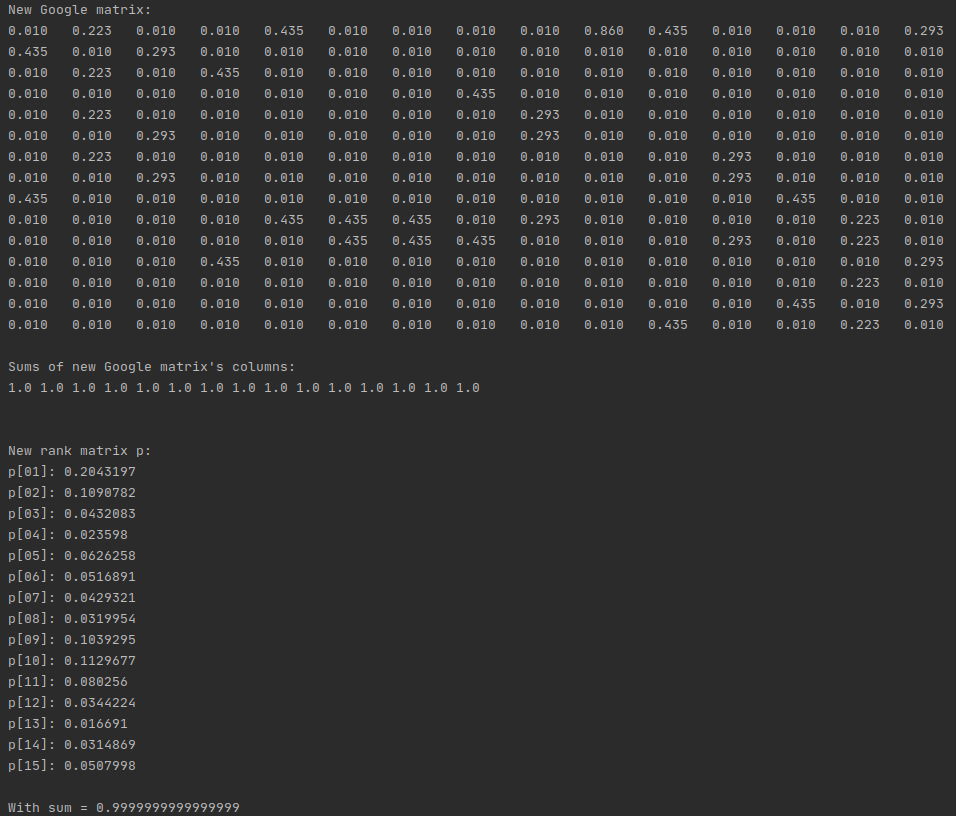
\includegraphics[width=\linewidth]{Exercise5/run_c.png}\\

Παραπάνω βλέπουμε ότι για:\\
\begin{itemize}
    \item {\lt $x = -\pi$} έχω προσέγγιση -0.674381 και απόλυτο σφάλμα $0.674381$
    \item {\lt $x = -\dfrac{7}{9}\pi$} έχω προσέγγιση -0.524519 και απόλυτο σφάλμα $0.118269$
    \item {\lt $x = -\dfrac{5}{9}\pi$} έχω προσέγγιση -0.374656 και απόλυτο σφάλμα $0.610152$
    \item {\lt $x = -\dfrac{\pi}{3}$} έχω προσέγγιση -0.224794 και απόλυτο σφάλμα $0.641232$
    \item {\lt $x = -\dfrac{\pi}{9}$} έχω προσέγγιση -0.074931 και απόλυτο σφάλμα $0.267089$
    \item {\lt $x = \dfrac{\pi}{9}$} έχω προσέγγιση 0.074931 και απόλυτο σφάλμα $0.267089$
    \item {\lt $x = \dfrac{\pi}{3}$} έχω προσέγγιση 0.224794 και απόλυτο σφάλμα $0.641232$
    \item {\lt $x = \dfrac{5}{9}\pi$} έχω προσέγγιση 0.374656 και απόλυτο σφάλμα $0.610152$
    \item {\lt $x = \dfrac{7}{9}\pi$} έχω προσέγγιση 0.524519 και απόλυτο σφάλμα $0.118269$
    \item {\lt $x = \pi$} έχω προσέγγιση 0.674381 και απόλυτο σφάλμα $0.674381$
\end{itemize}

Επομένως, στα <<γνωστά>> σημεία, έχουμε μεγαλύτερο απόλυτο σφάλμα για {\lt $x = -\pi, \pi$} με σφάλμα $0.674381 > 0$, επομένως στα <<γνωστά>> σημεία δεν έχουμε απαραίτητα κάποια δεκαδικά ψηφία ακρίβειας.

\par
Αν στην συνέχεια πάρουμε 200 σημεία ομοιόμορφα κατανεμημένα στο $[-\pi, \pi]$, υπολογίσουμε το απόλυτο σφάλμα, και εμφανίσουμε το σφάλμα αυτό κάθε σημείου σε διάγραμμα έχουμε το παρακάτω (υπολογίστηκε χρησιμοποιώντας την συνάρτηση {\lt scatter} του {\lt pyplot} της βιβλιοθήκης {\lt matplotlib} στο αρχείο {\lt c\textunderscore least\textunderscore squares\textunderscore approximation\textunderscore errors\textunderscore graph.py} που περιλαμβάνει τον ίδιο κώδικα με το αρχείο που περιγράφεται παραπάνω με διαφορετική όμως {\lt main} που αντί να χρησιμοποιεί τα δεδομένα σημεία, <<επιλέγει>> ομοιόμορφα κατανεμημένα 200 σημεία στο $[-\pi, \pi]$, υπολογίζει τις προσεγγίσεις κάθε ενός από τα αυτά και κατασκευάζει το διάγραμμα):\\

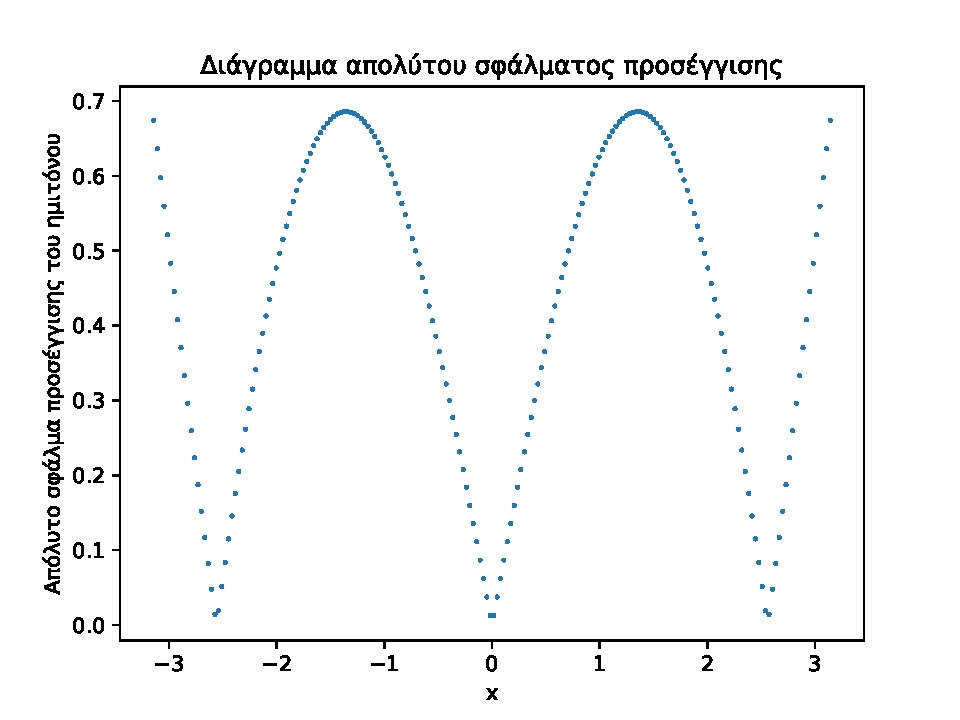
\includegraphics[width=\linewidth]{Exercise5/Figure_c.pdf}\\
Από το παραπάνω διάγραμμα μπορούμε να δούμε ότι στα 200 σημεία το μέγιστο απόλυτο σφάλμα ξεπερνάει το 0. Επομένως, δεν έχουμε απαραίτητα κάποια δεκαδικά ψηφία ακρίβειας σε κάθε ένα από αυτά τα 200 σημεία .

\section{Σύγκριση προσεγγίσεων}
Από την παραπάνω ανάλυση, μπορούμε να διαπιστώσουμε ότι, εν γένει στο $[-\pi, \pi]$, η μέθοδος πολυωνυμικής προσέγγισης είναι η πιο ακριβής, ακολουθεί η μέθοδος με {\lt splines} και η λιγότερο ακριβής είναι η μέθοδος προσέγγισης ελαχίστων τετραγώνων.

\end{document}
